\chapter{Limite Continuo}

En esta seccion voy a estudiar el comportamiento de la fucion $\zeta (s) $ en el limite $L \rightarrow \infty$, donde quedara definida por:

\begin{equation}
\zeta (s) = \int _{0} ^{\infty} \rho (x) x^{-2 s} dx
\end{equation}

Donde la $\rho(x) $ es la densidad de autovalores, para llegar a esta ecuacion, voy a utilizar la representacion integral de la funcion $\zeta$ en el plano complejo e integrar sobre un camino dado por la figura(REFERENCIAR), para eso voy a trabajar con mi aproximacion (REFERENCIAR)



Dependiendo si estoy arriba o abajo del eje real, voy a tener un termino exponencialmente creciente/decreciente en el limite $L \rightarrow \infty$ proveniente de $e ^{i z t}$

Voy a separar mi integral en una parte de arriba y una parte de abajo, en el termino de arriba del eje real obtengo:

\begin{equation}
\begin{array}{c}
\frac{1}{2 \pi i} \int _{\infty} ^{t0} 
\partial _z
Log
\left(
\frac{e ^{-2 i z  L } e ^{- \frac{i \alpha}{2 \lambda} Log[2 z  L]} }{\Gamma[1-\frac{i \alpha}{2 z }]} +
\frac{e ^{ \frac{i \alpha}{2 z } Log[2 z  L]} }{\Gamma[1+\frac{i \alpha}{2 z }]}
\right) d z \\
z = i t + \epsilon 
\end{array}
\end{equation}

Sacando factor comun de modo que me quede un termino exponencialmente decrenciente dentro del Logatirmo obtengo

\begin{equation}
\frac{1}{2 \pi i}  \int _{\infty} ^{t0} 
\partial _{z}
\left(
\frac{i\alpha}{2 z} Log[2 z L] - Log[\Gamma[1 + \frac{i \alpha}{2 z}]] +
Log[1- \epsilon _L ]
\right)
d z
\end{equation}

Donde $ \epsilon _L \rightarrow 0$ si $L \rightarrow \infty $ , entonces Logaritmo va a cero, quedando la integral final:

\begin{equation}
\begin{array}{c}
\zeta (s) = 
\frac{L}{\pi}
\int _ {x_0} ^{\infty} x ^{-2s} dx + \\
\frac{\alpha}{2 \pi } \int _{x_0} ^{\infty} 
\left(
\frac{-1}{ x ^2} -
\frac{Log[2 x L]}{x ^2}  -
\frac{1}{ x ^2 } 
\left(
\psi (1 + \frac{i \alpha}{2 x}) + \psi (1 - \frac{i \alpha}{2 x}) 
\right)
\right)
x ^{-2s} d x
\end{array}
\end{equation}



Relizando las integrales termino a termino obtengo

\begin{equation}
\begin{array}{c}
\zeta (s) = 
\frac{\alpha}{2 \pi} x _{0} ^{-2s-1}
\left( 
\frac{1}{(1+2s) ^2} +
\frac{Log[2 L x _0]}{1+2s} -
\frac{1}{1+2s}
\right) + 
\frac{L}{\pi} \frac{x _0 ^{-2s+1}}{2s-1}  \\
- \frac{\alpha}{2 \pi}
\int _{x_0} ^{\infty} 
\left(
\psi(1 + \frac{i \alpha}{2 x}) +
\psi(1 - \frac{i \alpha}{2 x} )
\right)
x ^{-2s-2}
dx
\end{array}
\end{equation}


Para calcular el ultimo termino hay distintos desarrollos en serie de la funcion $\psi $ que se pueden usar, yo voy a el desarrollo 

\begin{equation}
\begin{array}{cc}
\psi (1+ z ) = - \gamma + \sum _{n=2} ^{\infty} (-1) ^n \zeta (n) z ^{n-1} & |z| < 1
\end{array}
\end{equation}

El cual su radio de convergencia esta centrado alrededor de $x = 0$

La ultima integral queda expresada como:

\begin{equation}
\int _{x_0} ^{\infty}
\left(
-2 \gamma + 
2 \sum _{n=2} ^{\infty}
\zeta (2n+1) (-1) ^{n+1}
( \frac{\alpha}{2 x} ) ^{2n}
\right)
x ^{-2s-2} dx
\end{equation}

Quedando la funcion $\zeta _A (s) $ :

\begin{equation}
\begin{array}{c}
\zeta _A (s) = 
\frac{L x0 ^{-2s+1} }{2 \pi } \frac{1}{s- 1/2} + 
\frac{\alpha x0 ^{-2s-1} }{8 \pi } \frac{1}{(s+1/2) ^2} + \\
\frac{\alpha x0 ^{-2s-1} }{4 \pi } 
\left(
Log[2 L x_0] + \gamma - 1
\right)
\frac{1}{s+1/2} + \\
\frac{x_0 ^{-2s}}{2\pi} 
\sum _{n=1} ^{\infty} (-1) ^{n} \zeta (2n+1) 
( \frac{\alpha}{2 x0} ) ^{2n+1} \frac{1}{s+n+1/2}
\end{array}
\end{equation}

Para ver la energía de vacío hay que evaluar esta expresion en $s=-1/2$ y graficar su parte finita, tal como esta en la figura [ \ref{fig:vacio} ] donde estan los primeros 100 terminos de la serie, en funcion de $x = \alpha / x_0$ y la suma exacta de la serie al reemplazar $\zeta (2s+1) = 1$.

\begin{figure}
    \centering
    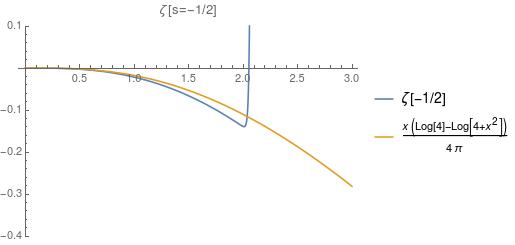
\includegraphics[scale=0.3]{Vacio.jpg}
    \caption{En esta imagen esta graficada la parte finita de la $\zeta _A (-1/2) $ en funcion del parametro $x= \frac{\alpha}{x _0}$ donde se sumaron los primeros 100 terminos de la serie, y en azul se puede ver la suma de la serie al reemplazar $\zeta (2n+1) = 1$}
    \label{fig:vacio}
\end{figure}